\setcounter{section}{22}
\section{LPC17xx System Tick Timer}

\subsection{Basic configuration}
\begin{itemize}
  \item \textbf{Clock source:} seleccionar \texttt{CCLK} interno o la entrada externa \texttt{STCLK} (\texttt{P3.26}) en \texttt{STCTRL}.
  \item \textbf{Pins:} si se usa \texttt{STCLK}, habilitar la funci\'on del pin correspondiente en el bloque de configuraci\'on de pines.
  \item \textbf{Interrupt:} habilitar la interrupci\'on del System Tick Timer en el \texttt{NVIC}.
\end{itemize}

\paragraph{Nota t\'ecnica}
El \texttt{SysTick} es parte integral del Cortex-M3 y usa un \textbf{vector de excepci\'on dedicado}. No es un perif\'erico externo del chip al estilo \texttt{UART} o \texttt{TIMER0}: es el temporizador est\'andar del n\'ucleo para base de tiempo peri\'odica.

\subsection{Features}
\begin{itemize}
  \item Intervalos de tiempo de \textbf{10 ms}.
  \item \textbf{Dedicated exception vector}.
  \item Puede tomar clock interno desde la CPU o externo desde el pin \texttt{STCLK}.
\end{itemize}

\subsection{Description}
\begin{itemize}
  \item El \texttt{System Tick Timer} est\'a pensado para generar una interrupci\'on fija cada \textbf{10 ms} para sistema operativo o software de gesti\'on del sistema.
  \item Al formar parte del Cortex-M3, facilita la portabilidad de software entre microcontroladores basados en ese n\'ucleo.
  \item El detalle arquitect\'onico fino de operaci\'on del \texttt{SysTick} se complementa con la gu\'ia del Cortex-M3 referida por el manual.
\end{itemize}

\subsection{Operation}
\begin{itemize}
  \item Es un temporizador de \textbf{24 bits} que cuenta hacia abajo hasta cero y genera una interrupci\'on.
  \item Puede tomar clock desde \texttt{CCLK} o desde \texttt{STCLK}.
  \item Para interrupciones peri\'odicas, \texttt{STRELOAD} debe cargarse con el valor de recarga correcto para el intervalo deseado.
  \item \texttt{STCALIB} trae un valor por defecto para \textbf{10 ms a 100 MHz}.
\end{itemize}

\begin{figure}[H]
  \centering
  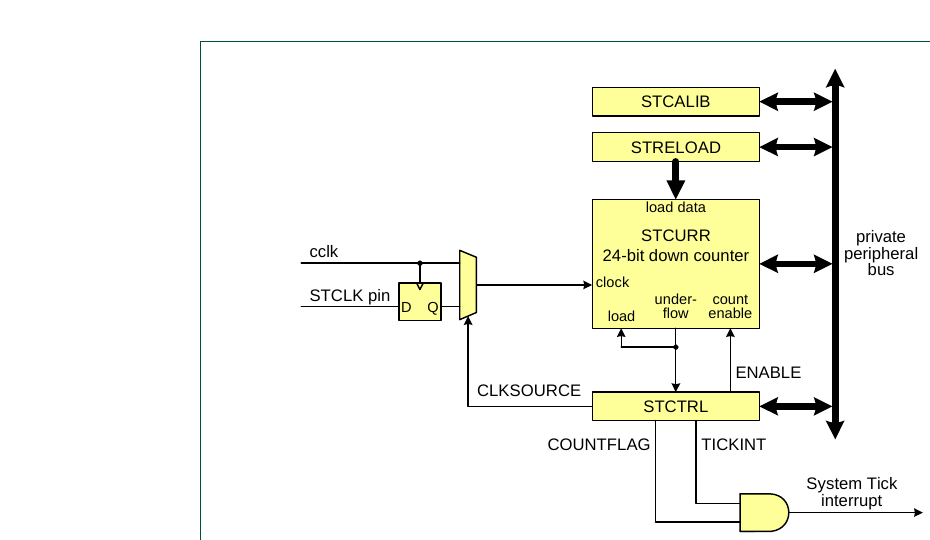
\includegraphics[width=0.90\textwidth]{images/lpc17xx_systick_block_diagram_fig118.png}
  \caption{System Tick Timer block diagram (Fig 118).}
\end{figure}

\paragraph{Nota t\'ecnica}
El flujo operativo real es: cargar \texttt{STRELOAD}, opcionalmente limpiar el contador escribiendo \texttt{STCURR}, configurar \texttt{STCTRL} y dejar que el contador recargue autom\'aticamente al llegar a cero. El bit \texttt{COUNTFLAG} se setea cuando ocurre ese underflow y se limpia al leer \texttt{STCTRL}.

\subsection{Register description}
\begin{table}[H]
  \centering
  \small
  \renewcommand{\arraystretch}{1.15}
  \caption{System Tick Timer register map (Table 438)}
  \begin{tabularx}{0.96\textwidth}{|>{\raggedright\arraybackslash}p{0.18\textwidth}|>{\raggedright\arraybackslash}X|>{\centering\arraybackslash}p{0.09\textwidth}|>{\centering\arraybackslash}p{0.14\textwidth}|>{\centering\arraybackslash}p{0.17\textwidth}|}
    \hline
    \textbf{Name} & \textbf{Description} & \textbf{Access} & \textbf{Reset value} & \textbf{Address} \\
    \hline
    \texttt{STCTRL} & System Timer Control and status register. & R/W & \texttt{0x4} & \texttt{0xE000 E010} \\
    \hline
    \texttt{STRELOAD} & System Timer Reload value register. & R/W & \texttt{0} & \texttt{0xE000 E014} \\
    \hline
    \texttt{STCURR} & System Timer Current value register. & R/W & \texttt{0} & \texttt{0xE000 E018} \\
    \hline
    \texttt{STCALIB} & System Timer Calibration value register. & R/W & \texttt{0x000F 423F} & \texttt{0xE000 E01C} \\
    \hline
  \end{tabularx}
\end{table}

\paragraph{Nota t\'ecnica}
El valor de reset reportado aplica a los \textbf{bits usados}. No debe interpretarse como contenido significativo en bits reservados.

\subsubsection{System Timer Control and status register (\texttt{STCTRL} - \texttt{0xE000 E010})}
\begin{table}[H]
  \centering
  \small
  \renewcommand{\arraystretch}{1.15}
  \caption{System Timer Control and status register (\texttt{STCTRL} - \texttt{0xE000 E010}) bit description (Table 439)}
  \begin{tabularx}{0.96\textwidth}{|>{\centering\arraybackslash}p{0.10\textwidth}|>{\raggedright\arraybackslash}p{0.18\textwidth}|>{\raggedright\arraybackslash}X|>{\centering\arraybackslash}p{0.12\textwidth}|}
    \hline
    \textbf{Bit} & \textbf{Symbol} & \textbf{Description} & \textbf{Reset value} \\
    \hline
    0 & \texttt{ENABLE} & Habilita el contador SysTick. \texttt{1}: contador habilitado. \texttt{0}: contador deshabilitado. & \texttt{0} \\
    \hline
    1 & \texttt{TICKINT} & Habilita la interrupci\'on del SysTick. Si vale \texttt{1}, la interrupci\'on se genera cuando el contador llega a \texttt{0}. & \texttt{0} \\
    \hline
    2 & \texttt{CLKSOURCE} & Selecci\'on de clock. \texttt{1}: \texttt{CPU clock}. \texttt{0}: pin externo \texttt{STCLK}. & \texttt{1} \\
    \hline
    15:3 & --- & Reservado. Software de usuario no debe escribir \texttt{1} en bits reservados. El valor le\'ido no est\'a definido. & \texttt{NA} \\
    \hline
    16 & \texttt{COUNTFLAG} & Flag que se setea cuando el contador llega a \texttt{0}. Se limpia al leer este registro. & \texttt{0} \\
    \hline
    31:17 & --- & Reservado. Software de usuario no debe escribir \texttt{1} en bits reservados. El valor le\'ido no est\'a definido. & \texttt{NA} \\
    \hline
  \end{tabularx}
\end{table}

\paragraph{Uso pr\'actico}
Si se usa como \textit{tick} peri\'odico, una configuraci\'on t\'ipica para clock interno es \texttt{ENABLE=1}, \texttt{TICKINT=1}, \texttt{CLKSOURCE=1}, lo que deja \texttt{STCTRL = 7}.

\subsubsection{System Timer Reload value register (\texttt{STRELOAD} - \texttt{0xE000 E014})}
\begin{table}[H]
  \centering
  \small
  \renewcommand{\arraystretch}{1.15}
  \caption{System Timer Reload value register (\texttt{STRELOAD} - \texttt{0xE000 E014}) bit description (Table 440)}
  \begin{tabularx}{0.96\textwidth}{|>{\centering\arraybackslash}p{0.10\textwidth}|>{\raggedright\arraybackslash}p{0.18\textwidth}|>{\raggedright\arraybackslash}X|>{\centering\arraybackslash}p{0.12\textwidth}|}
    \hline
    \textbf{Bit} & \textbf{Symbol} & \textbf{Description} & \textbf{Reset value} \\
    \hline
    23:0 & \texttt{RELOAD} & Valor que se carga en el contador SysTick cuando cuenta hacia abajo hasta \texttt{0}. & \texttt{0} \\
    \hline
    31:24 & --- & Reservado. Software de usuario no debe escribir \texttt{1} en bits reservados. El valor le\'ido no est\'a definido. & \texttt{NA} \\
    \hline
  \end{tabularx}
\end{table}

\subsubsection{System Timer Current value register (\texttt{STCURR} - \texttt{0xE000 E018})}
\begin{table}[H]
  \centering
  \small
  \renewcommand{\arraystretch}{1.15}
  \caption{System Timer Current value register (\texttt{STCURR} - \texttt{0xE000 E018}) bit description (Table 441)}
  \begin{tabularx}{0.96\textwidth}{|>{\centering\arraybackslash}p{0.10\textwidth}|>{\raggedright\arraybackslash}p{0.18\textwidth}|>{\raggedright\arraybackslash}X|>{\centering\arraybackslash}p{0.12\textwidth}|}
    \hline
    \textbf{Bit} & \textbf{Symbol} & \textbf{Description} & \textbf{Reset value} \\
    \hline
    23:0 & \texttt{CURRENT} & La lectura devuelve el valor actual del contador SysTick. Escribir cualquier valor limpia el contador SysTick y tambi\'en el bit \texttt{COUNTFLAG} en \texttt{STCTRL}. & \texttt{0} \\
    \hline
    31:24 & --- & Reservado. Software de usuario no debe escribir \texttt{1} en bits reservados. El valor le\'ido no est\'a definido. & \texttt{NA} \\
    \hline
  \end{tabularx}
\end{table}

\paragraph{Nota t\'ecnica}
\texttt{STCURR} no se usa para ``cargar'' un valor de arranque fino; para eso se usa \texttt{STRELOAD}. Su funci\'on operativa m\'as importante es permitir leer el conteo actual o forzar una limpieza del contador y del \texttt{COUNTFLAG}.

\subsubsection{System Timer Calibration value register (\texttt{STCALIB} - \texttt{0xE000 E01C})}
\begin{table}[H]
  \centering
  \small
  \renewcommand{\arraystretch}{1.15}
  \caption{System Timer Calibration value register (\texttt{STCALIB} - \texttt{0xE000 E01C}) bit description (Table 442)}
  \begin{tabularx}{0.96\textwidth}{|>{\centering\arraybackslash}p{0.10\textwidth}|>{\raggedright\arraybackslash}p{0.16\textwidth}|>{\raggedright\arraybackslash}p{0.18\textwidth}|>{\raggedright\arraybackslash}X|>{\centering\arraybackslash}p{0.12\textwidth}|}
    \hline
    \textbf{Bit} & \textbf{Symbol} & \textbf{Value} & \textbf{Description} & \textbf{Reset value} \\
    \hline
    23:0 & \texttt{TENMS} & --- & Valor de recarga para obtener un underflow SysTick cada \textbf{10 ms} cuando el clock es \textbf{100 MHz}. Los valores de \texttt{TENMS}, \texttt{SKEW} y \texttt{NOREF} aplican a ese caso de referencia. & \texttt{0x0F 423F} \\
    \hline
    29:24 & --- & --- & Reservado. Software de usuario no debe escribir \texttt{1} en bits reservados. El valor le\'ido no est\'a definido. & \texttt{NA} \\
    \hline
    30 & \texttt{SKEW} & --- & Indica si el valor de \texttt{TENMS} genera un intervalo exacto de \textbf{10 ms} o una aproximaci\'on. \texttt{0}: preciso. \texttt{1}: no preciso. & \texttt{0} \\
    \hline
    31 & \texttt{NOREF} & --- & Indica si existe clock de referencia externo separado. \texttt{0}: hay referencia separada disponible. \texttt{1}: no hay referencia separada. & \texttt{0} \\
    \hline
  \end{tabularx}
\end{table}

\paragraph{Nota t\'ecnica}
\texttt{STCALIB} no reemplaza el c\'alculo de \texttt{STRELOAD} para cualquier frecuencia arbitraria. Sirve como referencia de f\'abrica para el caso de \textbf{100 MHz}, que es el uso can\'onico que ARM asocia a SysTick.

\subsection{Example timer calculations}
\begin{table}[H]
  \centering
  \small
  \renewcommand{\arraystretch}{1.15}
  \caption{Resumen de c\'alculos de temporizaci\'on para \texttt{SysTick} a 10 ms}
  \begin{tabularx}{0.96\textwidth}{|>{\raggedright\arraybackslash}p{0.11\textwidth}|>{\raggedright\arraybackslash}p{0.22\textwidth}|>{\raggedright\arraybackslash}p{0.12\textwidth}|>{\raggedright\arraybackslash}p{0.19\textwidth}|>{\raggedright\arraybackslash}X|}
    \hline
    \textbf{Ejemplo} & \textbf{Clock} & \textbf{\texttt{STCTRL}} & \textbf{\texttt{RELOAD}} & \textbf{Observaci\'on} \\
    \hline
    1 & \texttt{CCLK = 100 MHz} & \texttt{7} & \texttt{999999 = 0xF423F} & Sin error de redondeo; coincide con el uso previsto del \texttt{STCALIB}. \\
    \hline
    2 & \texttt{CCLK = 80 MHz} & \texttt{7} & \texttt{799999 = 0xC34FF} & Sin error de redondeo; la precisi\'on depende de \texttt{CCLK}. \\
    \hline
    3 & \texttt{FIRC = 4 MHz} & \texttt{7} & \texttt{39999 = 0x9C3F} & Sin error de redondeo; la precisi\'on depende del \texttt{IRC}. \\
    \hline
    4 & \texttt{STCLK = 32.768 kHz} & \texttt{3} & \texttt{327 = 0x0147} & Hay error de redondeo; la frecuencia de interrupci\'on deriva levemente respecto del clock de entrada. \\
    \hline
  \end{tabularx}
\end{table}

\paragraph{Uso pr\'actico}
Para un per\'iodo objetivo de \textbf{10 ms}, la regla del manual es \texttt{RELOAD = (f / 100) - 1}. Cuando la frecuencia no es m\'ultiplo exacto de \texttt{100}, el resultado debe redondearse y eso introduce deriva temporal.
